\section{Experiments}
\label{sec:experiments}

Our experimental analysis addresses five questions:
%
How does CORELS' accuracy compare to that of other algorithms,
including COMPAS scores? (\S\ref{sec:sparsity})
%
How does CORELS' model size compare to that of other algorithms? (\S\ref{sec:sparsity})
%
How rapidly do the objective value and its lower bound converge,
for different values of the regularization parameter~$\Reg$? (\S\ref{sec:reg-param})
%
How much does each of the implementation optimizations contribute to CORELS' performance? (\S\ref{sec:ablation})
%
How rapidly does CORELS prune the search space? (\S\ref{sec:reg-param} and \S\ref{sec:ablation})
%
Before proceeding to the analysis described above,
we first describe our computational environment, as well as
datasets we use and prediction problems for each,
and then show example optimal rule lists found by CORELS (\S\ref{sec:examples}).

\textbf{Computational environment.}
%\label{sec:environment}
All timed results ran on a server with 44 Intel Xeon E5-2699~v4 (56~MB cache, 2.20GHz) and 251~GB RAM.
%with two Intel Xeon E5-2699~v4 (55~MB cache, 2.20~GHz) processors and 756~GB RAM.
%
Except where we mention a memory constraint, all experiments
can run comfortably on smaller machines, \eg a laptop with 16GB~RAM.

%\textbf{Datasets and prediction problems.}
%\label{sec:datasets}
Our evaluation focuses on two socially-important prediction problems associated
with recent, publicly-available datasets.

\textbf{ProPublica recidivism dataset.}
For our first problem, we predict which individuals in the ProPublica COMPAS
dataset~\citep{LarsonMaKiAn16} recidivate within two years.
This dataset contains records for all offenders in Broward County, Florida
in 2013 and 2014 who were given a COMPAS score pre-trial.
Recidivism is defined as committing a crime within 2 years of the COMPAS
assessment.
This dataset contains records for 7,214 individuals, of which we had complete data for 6,907 of them.
%
For the majority of our analysis, we extract a set of 14 features,
which our antecedent mining framework combines into ${M=122}$ antecedents,
on average (folds ranged from containing 121 to 123 antecedents).
%
We also consider a second, similar antecedent set in~\S\ref{sec:examples}.

\textbf{NYCLU stop-and-frisk dataset.} For our second problem, we use
the NYCLU 2014 stop-and-frisk dataset~\citep{nyclu:2014} to predict
whether a weapon will be found on a stopped individual who is frisked or searched.
%
From the original dataset of 45,787 records, each describing an incident involving
a stopped person, we identify a subset of 29,595 records for which the individual
was frisked and/or searched.
%
Of these, criminal possession of a weapon was identified in only about 5\% of instances.
%
Resampling due to class imbalance, for 10-fold cross-validation, yields training sets
that each contain 50,743 datapoints.
%
From a set of 5 categorical features, we form a set of ${M=46}$ single-clause antecedents (including negations)
that we use in our experiments below.

For further details about these datasets, preprocessing steps, and antecedent mining,
see Appendix~\ref{appendix:data}.
%
Our choice of, and approach to, the weapon prediction problem is inspired by the work
of~\citet{Goel16}, who develop regression models to analyze racial disparities
in New York City's stop-and-frisk policy for a similar, but larger, dataset.
%
In particular, the authors arrive at a simple and interpretable heuristic that
could potentially help police officers more effectively decide when to
frisk and/or search stopped individuals, \ie when such
interventions are likely to discover criminal possession of a weapon.

\subsection{Example optimal rule lists}
\label{sec:examples}

To motivate the feature set we used in most of our analysis of the ProPublica dataset,
described in Appendix~\ref{appendix:data}, we first consider a slightly different feature set.

%
\begin{figure}[t!]
\begin{algorithmic}
\State \bif $(age = 21-22) \band (priors = 2-3)$ \bthen $yes$
\State \belif $(age = 18-20)\band (sex = male)$ \bthen $yes$
\State \belif $(priors > 3)$ \bthen $yes$
\State \belse $no$
\end{algorithmic}
\vspace{1mm}
\begin{algorithmic}
\State \bif $(age = 23-25) \band (priors = 2-3)$ \bthen $yes$
\State \belif $(age = 18-20)\band (sex = male)$ \bthen $yes$
\State \belif $(age = 21-22) \band (priors = 2-3)$ \bthen $yes$
\State \belif $(priors > 3)$ \bthen $yes$
\State \belse $no$
\end{algorithmic}
\caption{Two representative optimal rule lists that predict two-year recidivism for the
ProPublica dataset, found by CORELS (${\Reg = 0.005}$), across 10 cross-validation folds.
%
The remaining 8 optimal rule lists were the same or similar to these two lists, with prefixes containing the same rules, up to a permutation,
and the same default rules.
}
\label{fig:propublica}
\end{figure}
%
\begin{figure}[hb!]
\vspace{1mm}
\begin{algorithmic}
\State \bif $(age = 18-20)\band (sex = male)$ \bthen $yes$
\State \belif $(age = 21-22) \band (priors = 2-3)$ \bthen $yes$
\State \belif $(priors > 3)$ \bthen $yes$
\State \belse $no$
\end{algorithmic}
\vspace{1mm}
\begin{algorithmic}
\State \bif $(age = 21-22) \band (priors = 2-3)$ \bthen $yes$
\State \bif $(age = 23-25) \band (priors = 2-3)$ \bthen $yes$
\State \belif $(priors > 3)$ \bthen $yes$
\State \belif $(sex = male) \band (age = 18-20)$ \bthen $yes$
\State \belse $no$
\end{algorithmic}
\caption{Example optimal rule lists that predict two-year recidivism for the
ProPublica dataset, found by CORELS, across 10 cross-validation folds.
%
All other rule lists found contained the same rules as these two lists, though the prefix order was permuted.
%
We observe that while these rule lists are not identical to the ones found in the earlier dataset, they contain
the same rules as the dataset that included race features
%
Additionally, all of these rule lists start with the same rule,
end with the same default rule, and contain the same prefix rules, up to a permutation;
the prefix rules always predict the positive class label,
and the default rule always predicts the negative class label.
%
Thus, these rule lists could be equivalently expressed as a DNF rule.
%
Note that our objective is not designed to enforce any of these properties,
though some may be seen as desirable.
}
\label{fig:recidivism-all-folds}
\end{figure}
%
Figure~\ref{fig:propublica} shows optimal rule lists learned by CORELS,
using a feature set that includes the race categories from the ProPublica dataset (African American, Caucasian, Hispanic,
Other\footnote{We grouped together the original Native American ($<$0.003), Asian ($<$0.005), and Other ($<$0.06) categories.}).
%
For this feature set, our antecedent mining procedure generated an average
of~189 antecedents, across folds.
%
Notice that none of these rule lists contain antecedents that directly depend on race;
this motivated our choice to exclude race in our subsequent analysis.
%
For both versions of the dataset, we chose a set of age ranges that was fine-grained
for younger individuals (18-20, 21-22, 23-25, 26-45, $>$45), as opposed to the original ProPublica categories of ($<$25, 25-45, $>$45).

\begin{figure}[t!]
\begin{algorithmic}
\State \bif $(location = transit~authority)$ \bthen $yes$
\State \belif $(stop~reason = suspicious~object)$ \bthen $yes$
\State \belif $(stop~reason = suspicious~bulge)$ \bthen $yes$
\State \belse $no$
\end{algorithmic}
\caption{An example rule list that predicts whether a weapon will be found on a
stopped individual who is frisked or searched, for the NYCLU stop-and-frisk dataset.
%
This is the most common optimal rule list found by CORELS across 10 cross-validation
folds; the others contain the same rules, up to a permutation.
}
\label{fig:weapon-rule-list}
\end{figure}

Figures~\ref{fig:recidivism-all-folds} and~\ref{fig:weapon-rule-list}
show example optimal rule lists that CORELS learns
for the ProPublica (${\Reg = 0.005}$) and NYCLU (${\Reg = 0.01}$) datasets, respectively,
using 10-fold cross validation and the antecedent sets described
at the beginning of~\S\ref{sec:experiments}.

While our goal is to provide illustrative examples, and not to provide a
detailed analysis nor to advocate for the use of these specific models,
we note that these rule lists are short and easy to understand.
%
Furthermore, as we demonstrate in~\S\ref{sec:sparsity},
optimal rule lists learned by CORELS achieve accuracies that are competitive
with a suite of other models, including black box COMPAS scores.
%
We also note that the three-rule list for weapon prediction
in Figure~\ref{fig:weapon-rule-list} has the spirit of the heuristic
strategy presented by~\citet{Goel16} that combines three stop criteria
and is based on a reduced version of their full regression model.
%
See Appendix~\ref{appendix:examples} for additional listings of optimal rule lists found
by CORELS, for each of our prediction problems, across cross-validation folds,
for different values of the regularization parameter~$\Reg$.

\subsection{Comparison of accuracy and model size for CORELS and other algorithms}
\label{sec:sparsity}

We ran a 10-fold cross validation experiment using CORELS
and eight other algorithms:
logistic regression, support vector machines, AdaBoost, CART, C4.5,
random forests, RIPPER, and scalable Bayesian rule lists (SBRL).\footnote{For
SBRL, we use the C implementation at \url{https://github.com/Hongyuy/sbrlmod}.
By default, SBRL sets ${\eta = 3}$, ${\lambda = 9}$,
the number of chains to 11 and iterations to 1,000.}
%
We use standard R packages, with default parameter settings,
for the first seven algorithms.\footnote{For CART, C4.5 (J48), and RIPPER,
\ie the tree and rule list learning algorithms, we use the implementations
from the R packages rpart, RWeka, and caret, respectively.
%
By default, CART uses complexity parameter ${cp = 0.01}$,
and C4.5 uses complexity parameter ${C = 0.25}$.
}
%
We use the same antecedent sets as input to the two rule list learning algorithms, CORELS and SBRL;
for the other algorithms, the inputs are binary feature sets corresponding to the
single clause antecedents in the aforementioned antecedent sets (see Appendix~\ref{appendix:data}).

Figure~\ref{fig:comparison} shows that there were no statistically significant
differences in algorithm accuracies.
In fact, the difference between folds was far larger than the difference
between algorithms.
We conclude that CORELS produces models whose accuracy is comparable
to those found via other algorithms.

%TODO: REPLACE COMPARISON FIGURE
\begin{figure}[t!]
\begin{center}
%\includegraphics[width=0.75\textwidth]{figs/sketch-comparison.png}
% left lower right upper
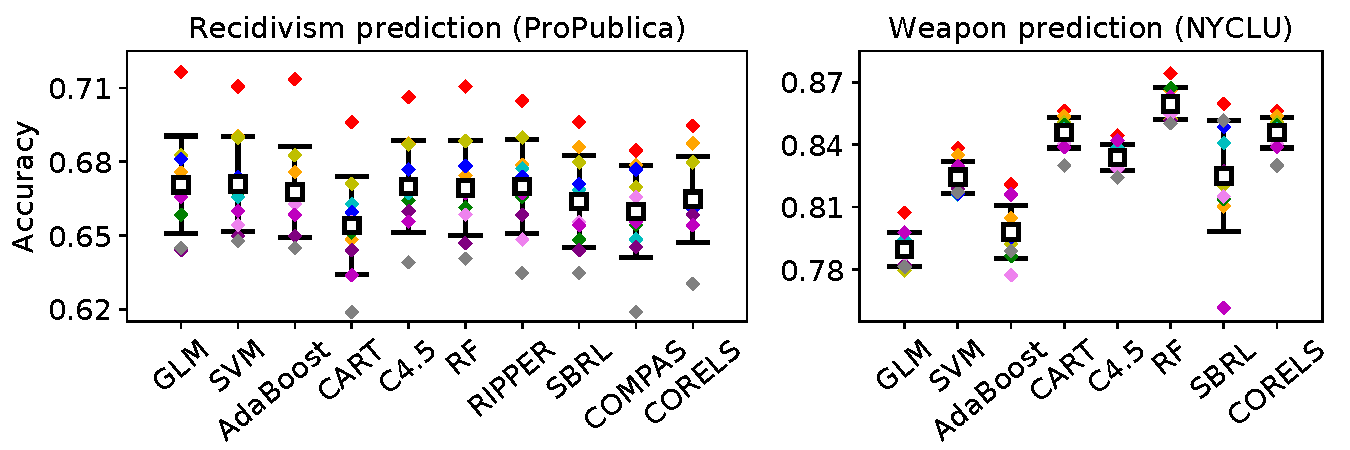
\includegraphics[trim={10mm, 5mm, 15mm, 5mm},
width=\textwidth]{figs/compare-compas-weapon.pdf}
\end{center}
\caption{Comparison of CORELS and a panel of eight other algorithms:
logistic regression~(GLM), support vector machines~(SVM),
AdaBoost, CART, C4.5, random forests~(RF), RIPPER,
scalable Bayesian rule lists~(SBRL).
%
Test accuracy means (white squares),
standard deviations (error bars),
and values (colors correspond to folds),
for 10-fold cross-validation experiments.
%
Left:~Two-year recidivism prediction for the ProPublica COMPAS dataset.
%
For CORELS, we use regularization parameter~${\Reg=0.005}$.
%
Right:~Weapon prediction for the NYCLU stop-and-frisk dataset.
%
For CORELS, we use~${\Reg=0.01}$.
%
Note that we were unable to execute RIPPER for the NYCLU problem.
}
\label{fig:comparison}
\end{figure}

%TODO: REPLACE SPARSITY FIGURE
\begin{figure}[t!]
\begin{center}
%\includegraphics[width=0.75\textwidth]{figs/sketch-comparison.png}
% left lower right upper
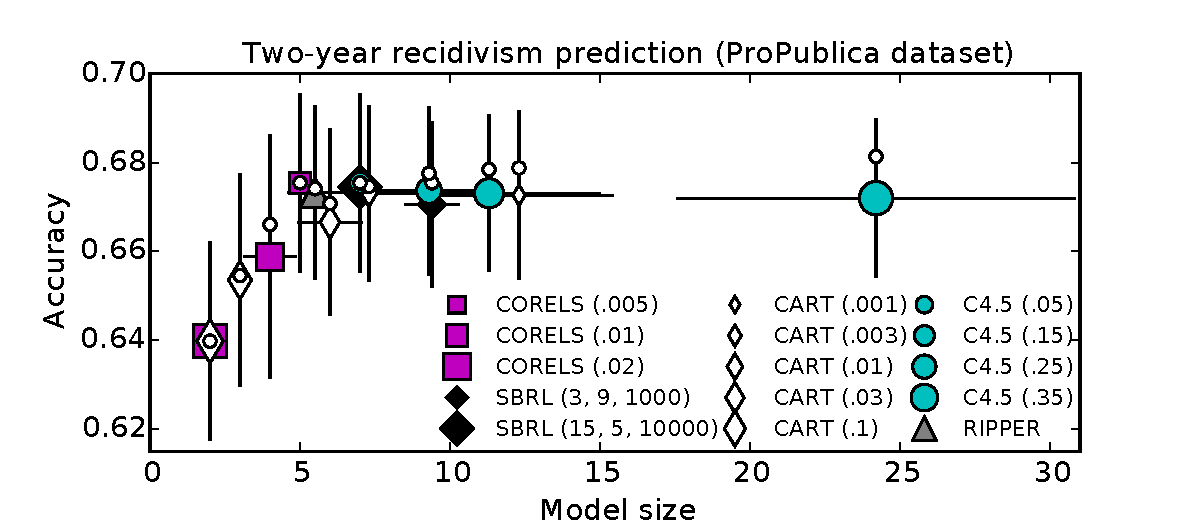
\includegraphics[trim={12mm, 0mm, 24mm, 5mm},
width=0.93\textwidth]{figs/compas-sparsity-training.pdf}
\vspace{6mm}

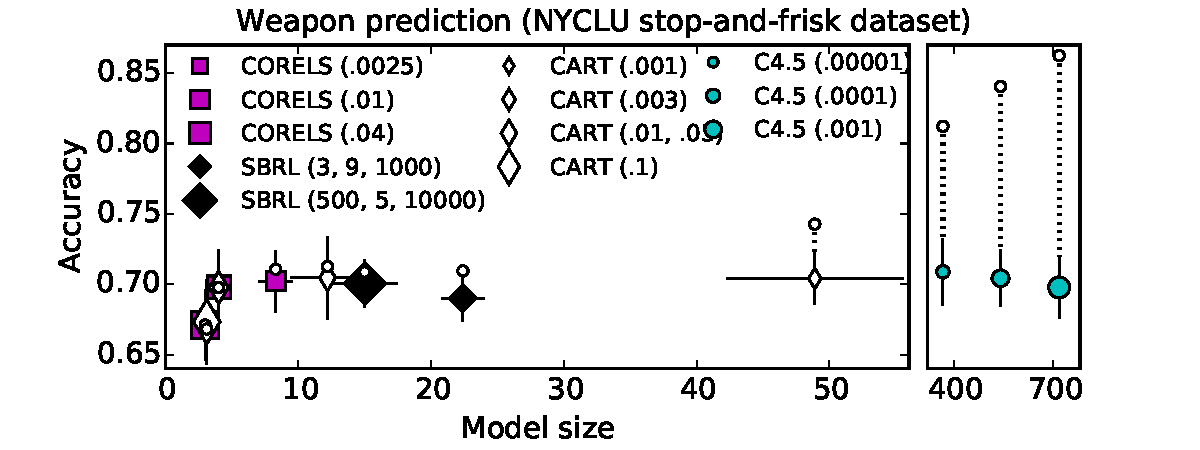
\includegraphics[trim={12mm, 0mm, 24mm, 0mm},
width=0.93\textwidth]{figs/frisk-sparsity-training-c45.pdf}
\end{center}
\caption{Training and test accuracy as a function of model size.
%
In the legend, numbers in parentheses are algorithm parameters that we vary
for CORELS~($\Reg$), CART~($cp$), C4.5~($C$), and SBRL ($\eta$, $\lambda$, $i$),
where~$i$ is the number of iterations.
%
Note that the CART implementation sets ${cp = 0.01}$ by default,
and C4.5 uses ${C = 0.25}$.
%
Legend markers and error bars indicate means and standard deviations,
respectively, of test accuracy across cross-validation folds.
%
Small circles mark associated training accuracy means.
%
Top:  Two-year recidivism prediction for the ProPublica COMPAS dataset.
%
%For CORELS and SBRL, the number of antecedents~$M$ is between 155 and 157.
%
None of the models exhibit significant overfitting --
mean training accuracy never exceeds mean test accuracy
by more than about 0.01.
%
Bottom:  Weapon prediction for the NYCLU stop-and-frisk dataset.
%
%For CORELS and SBRL, we use ${M = 28}$ antecedents.
%
CART with ${cp = 0.001}$ significantly overfits;
C4.5 finds large models and dramatically overfits for all tested parameters.
}
\label{fig:sparsity}
\end{figure}

Figure~\ref{fig:sparsity} summarizes differences in accuracy and model size
for CORELS and other tree (CART, C4.5) and rule list (RIPPER, SBRL) learning algorithms.
%
Here, we vary different algorithm parameters, and increase the number of iterations for SBRL to 10,000.
%
For both problems, CORELS can learn short rule lists without sacrificing accuracy.
%
For listings of example optimal rule lists that correspond to the results
for CORELS summarized in Figure~\ref{fig:sparsity}, see Appendix~\ref{appendix:examples}.

%TODO, fix TEST ACCURACIES
\textbf{Comparison to COMPAS.}
The accuracies of rule lists learned by CORELS are competitive with
scores generated by the black box COMPAS algorithm
at predicting two-year recidivism for the ProPublica dataset.
%
Across 10 cross-validation folds, optimal rule lists learned by CORELS
(Figure~\ref{fig:recidivism-all-folds}, ${\Reg = 0.005}$)
have mean test accuracy~0.676, with standard deviation~0.020.
%
For comparison, optimal rule lists learned by CORELS,
for a slightly different feature set (Figure~\ref{fig:propublica}, ${\Reg = 0.005}$),
achieve a similar mean test accuracy of~0.659, with standard deviation~0.016, across folds.

The COMPAS algorithm outputs scores between~1 and~10,
representing low (1-4), medium (5-7), and high (8-10) risk for recidivism.
%
As in the analysis by~\citep{LarsonMaKiAn16}, we interpret a medium or high score
as a positive prediction for two-year recidivism, and a low score as a negative prediction.
%
Across the 10 test sets, the COMPAS algorithm scores obtain
mean accuracy of~0.654, with standard deviation~0.015.

In addition, we observe that CORELS achieves a lower FPR on black individuals than COMPAS does across all 10 folds.
%
While CORELS also has a lower TPR on black individuals than COMPAS, the two algorithms perform similarly on white individuals.
%
Both algorithms have much higher FPRs and TPRs on black individuals than white individuals.
%
Since the rule lists output by CORELS do not explicitly contain race, the rules involving prior criminal convictions must implicitly be racially skewed.
%
Although CORELS is less likely to predict a false positive for black individuals in this case, our primary advantage comes from the fact that our model can be easily inspected to determine why the prediction rates are different across races (or any other category).

\begin{figure}[t!]
% left lower right upper
\begin{center}
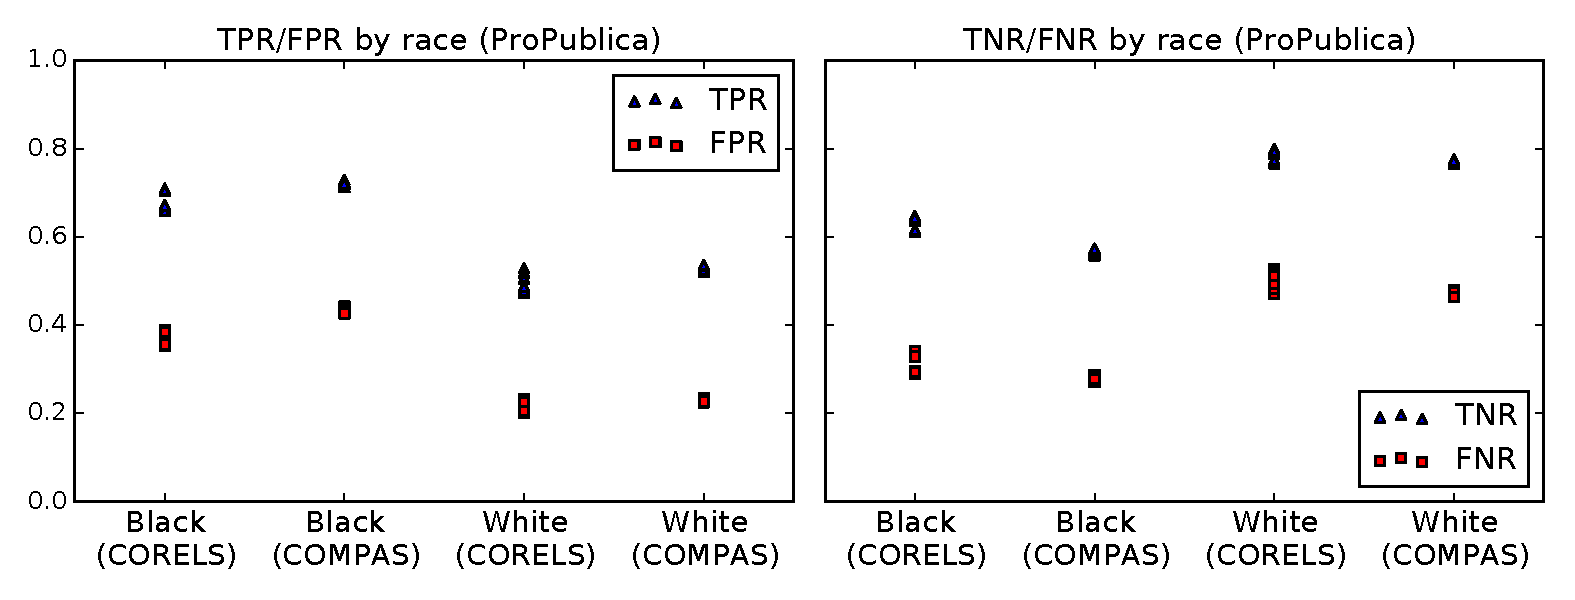
\includegraphics[trim={12mm, 0mm, 24mm, 0mm},
width=0.93\textwidth]{figs/compas-corels-comparison.pdf}
\end{center}
\caption{TPR and FPR of CORELS and COMPAS on the different races in our dataset across the 10 folds.
%
CORELS has a lower FPR on black individuals in the dataset than COMPAS, though it also has a slightly lower TPR.
%
Both CORELS and COMPAS have a significantly higher FPR rate for black indviduals than white individuals--despite CORELS producing optimal rule lists without explicit race features.
%
}
\label{fig:tpr-fpr}
\end{figure}

\subsection{CORELS execution traces, for different regularization parameters}
\label{sec:reg-param}
%TODO UPDATE ANALYSIS
In this section, we illustrate several views of CORELS execution traces,
for the NYCLU stop-and-frisk dataset with ${M = 46}$ antecedents,
for the same three regularization parameters (${\Reg = 0.04, 0.01, 0.025}$)
as in Figure~\ref{fig:sparsity} (bottom).

Table~\ref{tab:weapon-reg} summarizes execution traces across all 10 cross-validation folds.
%
For each value of~$\Reg$, CORELS achieves the optimum in a small fraction of the total execution time.
%
As~$\Reg$ decreases, these times increase because the search problems become more difficult,
as is summarized by the observation that CORELS must evaluate longer prefixes;
as a consequence, our data structures grow in size.
%
We report the total number of elements inserted into the queue and the maximum queue size;
recall from~\S\ref{sec:implementation} that the queue elements correspond to the trie's leaves,
and that the symmetry-aware map elements correspond to the trie's nodes.

The upper panels in Figure~\ref{fig:weapon-reg-execution} plot example execution traces,
from a single cross-validation fold, of both the current best objective value~$\CurrentObj$
and the lower bound~$b(\Prefix, \x, \y)$ of the prefix~$\Prefix$ being evaluated.
%
These plots illustrate that CORELS certifies optimality
when the lower bound matches the objective value.
%
The lower panels in Figure~\ref{fig:weapon-reg-execution} plot corresponding traces of
an upper bound on the size of the remaining search space (Theorem~\ref{thm:remaining-eval-fine}),
and illustrate that as~$\Reg$ decreases, it becomes more difficult to eliminate regions of the search~space.
%
For Figure~\ref{fig:weapon-reg-execution}, we dynamically and incrementally
calculate~$\lfloor \log_{10} \Remaining(\CurrentObj, \Queue) \rfloor$,
which adds some computational overhead; we do not perform this calculation elsewhere unless noted.

Figure~\ref{fig:queue-weapon-reg} visualizes the elements in CORELS's logical queue,
for each of the executions in Figure~\ref{fig:weapon-reg-execution}.
%
Recall from~\S\ref{sec:gc} that the logical queue corresponds to elements in the
(physical) queue that have not been garbage collected from the trie; these are prefixes that
CORELS has already evaluated and whose children the algorithm plans to evaluate next.
%
As an execution progresses, longer prefixes are placed in the queue;
as~$\Reg$ decreases, the algorithm must spend more time evaluating longer and longer prefixes.

\begin{table}[t!]
\centering
%\begin{centering}
CORELS with different regularization parameters (NYCLU stop-and-frisk dataset) \\
%\end{centering}
\vspace{2mm}
\begin{tabular}{l | c | c | c | c}
& Total & Time to & Max evaluated & Optimal \\
$\lambda$ & time (s) & optimum (s) & prefix length & prefix length \\
0.04 & 0.61 (0.03) & 0.002 (0.00046) & 6-6 & 2-2 \\
0.01 & 69.70 (6.09) & 0.008 (0.00162) & 11-11 & 3-3 \\
0.0025 & 1586.32 (108.04) & 56.321 (73.94361) & 16-17 & 6-10 \\
\hline
\end{tabular}
\begin{tabular}{l | c | c | c}
\hline
& Lower bound & Total queue &  Max queue \\
$\lambda$ & evaluations ($\times 10^6$) &~ insertions ($\times 10^3$) ~&~ size ($\times 10^3$) \\
\hline
0.04 & 0.070 (0.004) & 2.2 (0.1) & 0.94 (0.11) \\
0.01 & 7.532 (0.645) & 208.9 (18.4) & 134.90 (11.22) \\
0.0025 & 153.476 (10.416) & 4376.0 (302.7) & 2463.48 (173.11) \\
\end{tabular}
%\vspace{4mm}
\caption{Summary of CORELS executions, for the NYCLU stop-and-frisk dataset (${M = 46}$),
for same three regularization parameters as in Figure~\ref{fig:sparsity} (bottom).
%
The columns report the total execution time,
time to optimum, maximum evaluated prefix length, optimal prefix length,
number of times we completely evaluate a prefix~$\Prefix$'s lower bound~$b(\Prefix, \x, \y)$,
total number of queue insertions (which is equal to the number of cache insertions),
and the maximum queue size.
%
For prefix lengths, we report single values or ranges corresponding to the minimum and maximum observed values;
in the other columns, we report means (and standard deviations) over 10 cross-validation folds.
%
See also Figures~\ref{fig:weapon-reg-execution} and~\ref{fig:queue-weapon-reg}.
}
\vspace{4mm}
\label{tab:weapon-reg}
\end{table}

%TODO UPDATE FIGURE
\begin{figure}[t!]
\begin{center}
% left lower right upper
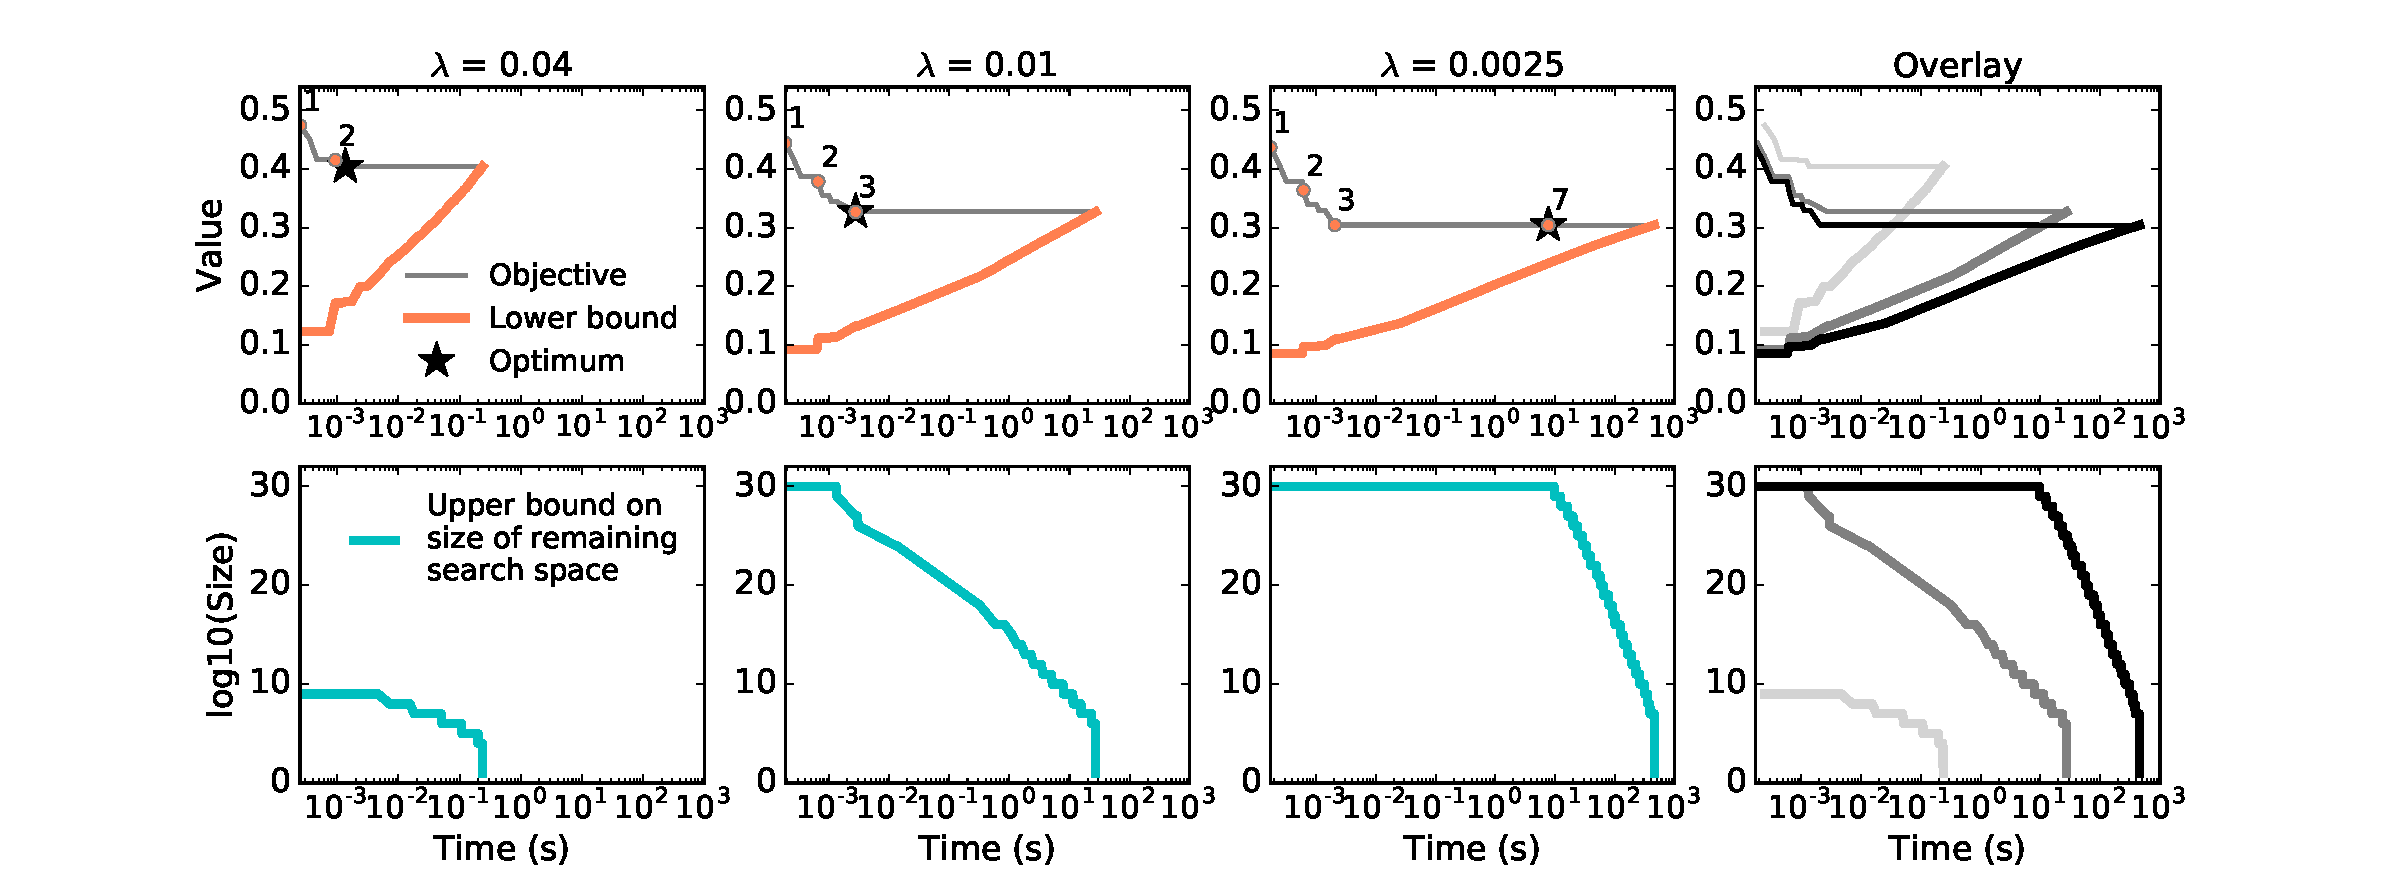
\includegraphics[trim={35mm 0mm 35mm 15mm},
width=0.97\textwidth]{figs/weapon_reg-execution.pdf}
\end{center}
\vspace{-5mm}
\caption{Example executions of CORELS, for the NYCLU stop-and-frisk dataset (${M = 46}$).
%
See also Table~\ref{tab:weapon-reg} and Figure~\ref{fig:queue-weapon-reg}.
%
Top: Objective value (thin line) and lower bound (thick line) for CORELS,
as a function of wall clock time (log scale).
%
Numbered points along the trace of the objective value
indicate when the length of the best known rule list changes
and are labeled by the new length.
%
For each value of~$\Reg$, a star marks the optimum objective value
and time at which it was achieved.
%
Bottom: $\lfloor \log_{10} \Remaining(\CurrentObj, \Queue) \rfloor$,
as a function of wall clock time (log scale),
where~$\Remaining(\CurrentObj, \Queue)$
is the upper bound on remaining search space size
(Theorem~\ref{thm:remaining-eval-fine}).
%
Rightmost panels: For visual comparison, we overlay the execution traces
from the panels to the left, for the three different values of~$\Reg$.
}
\label{fig:weapon-reg-execution}
\end{figure}

\begin{figure}[t!]
\begin{center}
% left lower right upper
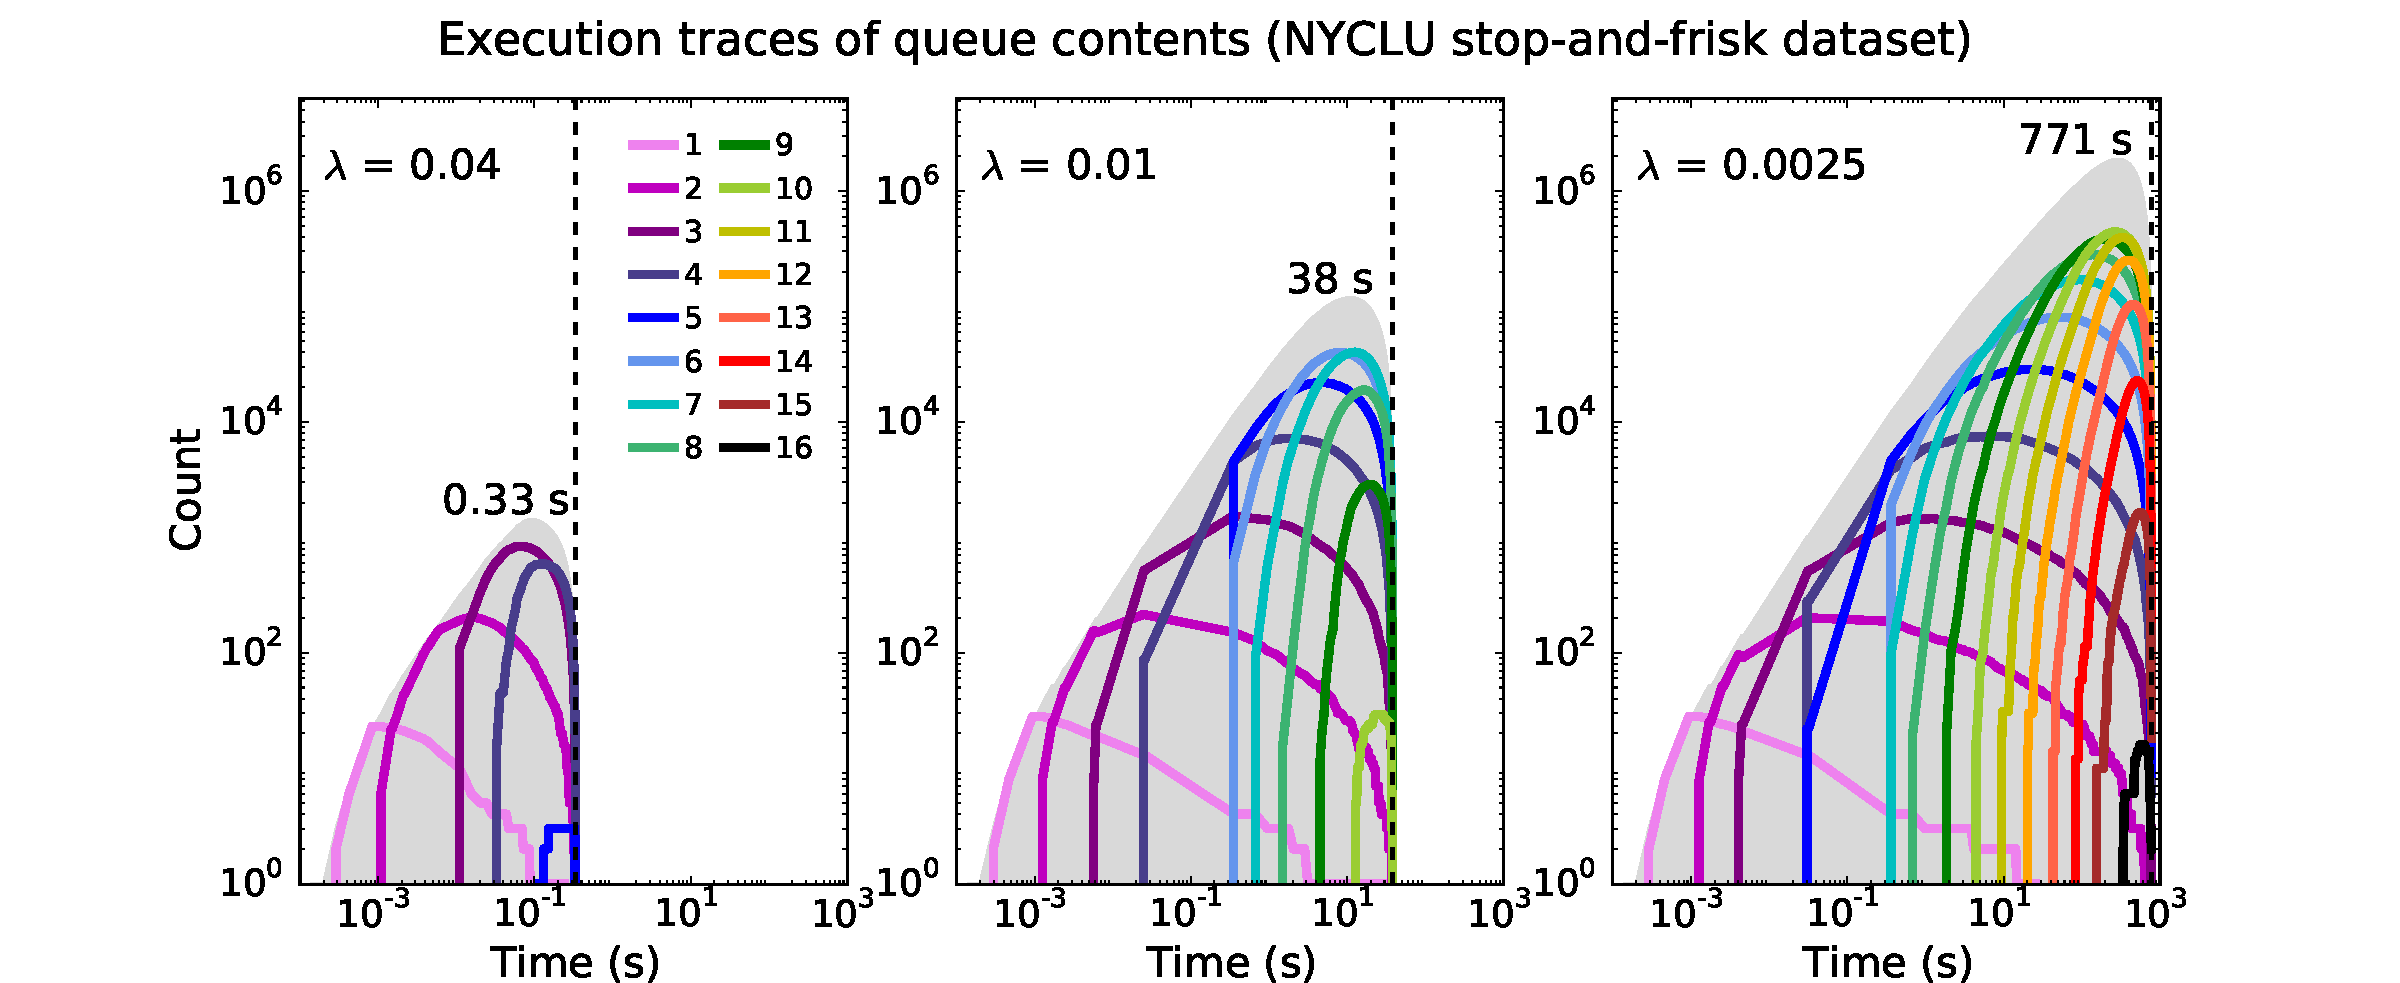
\includegraphics[trim={30mm 0mm 30mm 3mm},
width=0.9\textwidth]{figs/weapon_reg-queue.pdf}
\end{center}
\vspace{-5mm}
\caption{Summary of CORELS's logical queue,
%\ie the nodes in the physical queue that have not been marked for deletion,
for the NYCLU stop-and-frisk dataset (${M = 46}$),
for same three regularization parameters as in Figure~\ref{fig:sparsity} (bottom)
and Table~\ref{tab:weapon-reg}.
%
Solid lines plot the numbers of prefixes in the logical queue (log scale), colored by length (legend),
as a function of wall clock time (log scale).
%
All plots are generated using a single, representative cross-validation training set.
%
For each execution, the gray shading fills in the area beneath the total number
of queue elements, \ie the sum over all lengths;
we also annotate the total time in seconds, marked with a dashed vertical line.
}
\label{fig:queue-weapon-reg}
\end{figure}

\subsection{Efficacy of CORELS algorithm optimizations}
\label{sec:ablation}

This section examines the efficacy of each of our bounds and data structure optimizations.
%
We remove a single bound or data structure optimization from our final implementation and measure
how the performance of our algorithm changes.
%
We examine these performance traces on both the NYCLU and the ProPublica datasets,
and highlight that on different problems, the relative performance improvements of our optimizations can vary.

%\includegraphics[width=0.75\textwidth]{figs/sketch-ablation.png}
\begin{table}[t!]
\centering
%\begin{centering}
Per-component performance improvement (ProPublica dataset) \\
%\end{centering}
\vspace{1mm}
\begin{tabular}{l | c  r | c | c}
& Total time & Slow- & Time to & Max evaluated \\
Algorithm variant & (min) & down & optimum (s) & prefix length \\
\hline
CORELS & 0.98 (0.6) & --- & 1 (1) & 5-5 \\
No priority queue (BFS) & 1.03 (0.6) & 1.05$\times$ & 2 (4) & 5-5 \\
No support bounds & 1.49 (0.9) & 1.49$\times$ & 1 (2) & 5-5 \\
No lookahead bound & 12.28 (6.2) & 13.26$\times$ & 1 (1) & 6-6 \\
No symmetry-aware map & 9.11 (6.4) & 8.44$\times$ & 2 (3) & 5-5 \\
No equivalent points bound & $>$128.08 (2.6) & $>$184.89$\times$ & $>$1420 (2030) & $\ge$11 \\
\hline
\end{tabular}
\begin{tabular}{l | c | c | c}
\hline
 & Lower bound & Total queue &  Max queue \\
Algorithm variant & evaluations ($\times 10^6$) & insertions ($\times 10^6$) & size ($\times 10^6$) \\
\hline
CORELS & 26.04 (14.6) & 0.29 (0.2) & 0.24 (0.1) \\
No priority queue (BFS) & 27.23 (15.6) & 0.33 (0.2) & 0.20 (0.1) \\
No support bounds & 41.76 (25.2) & 0.40 (0.2) & 0.33 (0.2) \\
No lookahead bound & 318.82 (156.9) & 3.56 (1.8) & 3.04 (1.5) \\
No symmetry-aware map & 250.35 (175.2) & 2.45 (1.7) & 2.36 (1.7) \\
No equivalent points bound & $>$942.44 (4.7) & $>$508.51 (1.1) & $>$497.86 (1.2) \\
\end{tabular}
%\vspace{4mm}
\caption{Per-component performance improvement, for the ProPublica dataset
(${\Reg = 0.005}$, ${M = 123}$).
%
The columns report the total execution time,
time to optimum, maximum evaluated prefix length,
number of times we completely evaluate a prefix~$\Prefix$'s lower bound~$b(\Prefix, \x, \y)$,
total number of queue insertions (which is equal to the number of cache insertions),
and maximum logical queue size.
%
The first row shows CORELS; subsequent rows show variants
that each remove a specific implementation optimization or bound.
%
(We are not measuring the cumulative effects of removing a sequence of components.)
%
All rows represent complete executions, except for the final row,
in which each execution was terminated due to memory constraints,
once the size of the cache reached ${5 \times 10^8}$ elements,
after consuming $\sim$250GB RAM.
%
In all but the final row and column, we report means
(and standard deviations) over 10 cross-validation folds.
%
We also report the  mean slowdown in total execution time,
with respect to CORELS.
%
In the final row, we report the mean (and standard deviation) of the
incomplete execution time and corresponding slowdown,
and a lower bound on the mean time to optimum;
in the remaining fields, we report minimum values across folds.
%
See also Figure~\ref{fig:queue}. \\
%
*~Only 7 out of 10 folds achieve the optimum before being terminated.
}
\vspace{4mm}
\label{tab:ablation}
\end{table}

\begin{figure}[t!]
\begin{center}
% left lower right upper
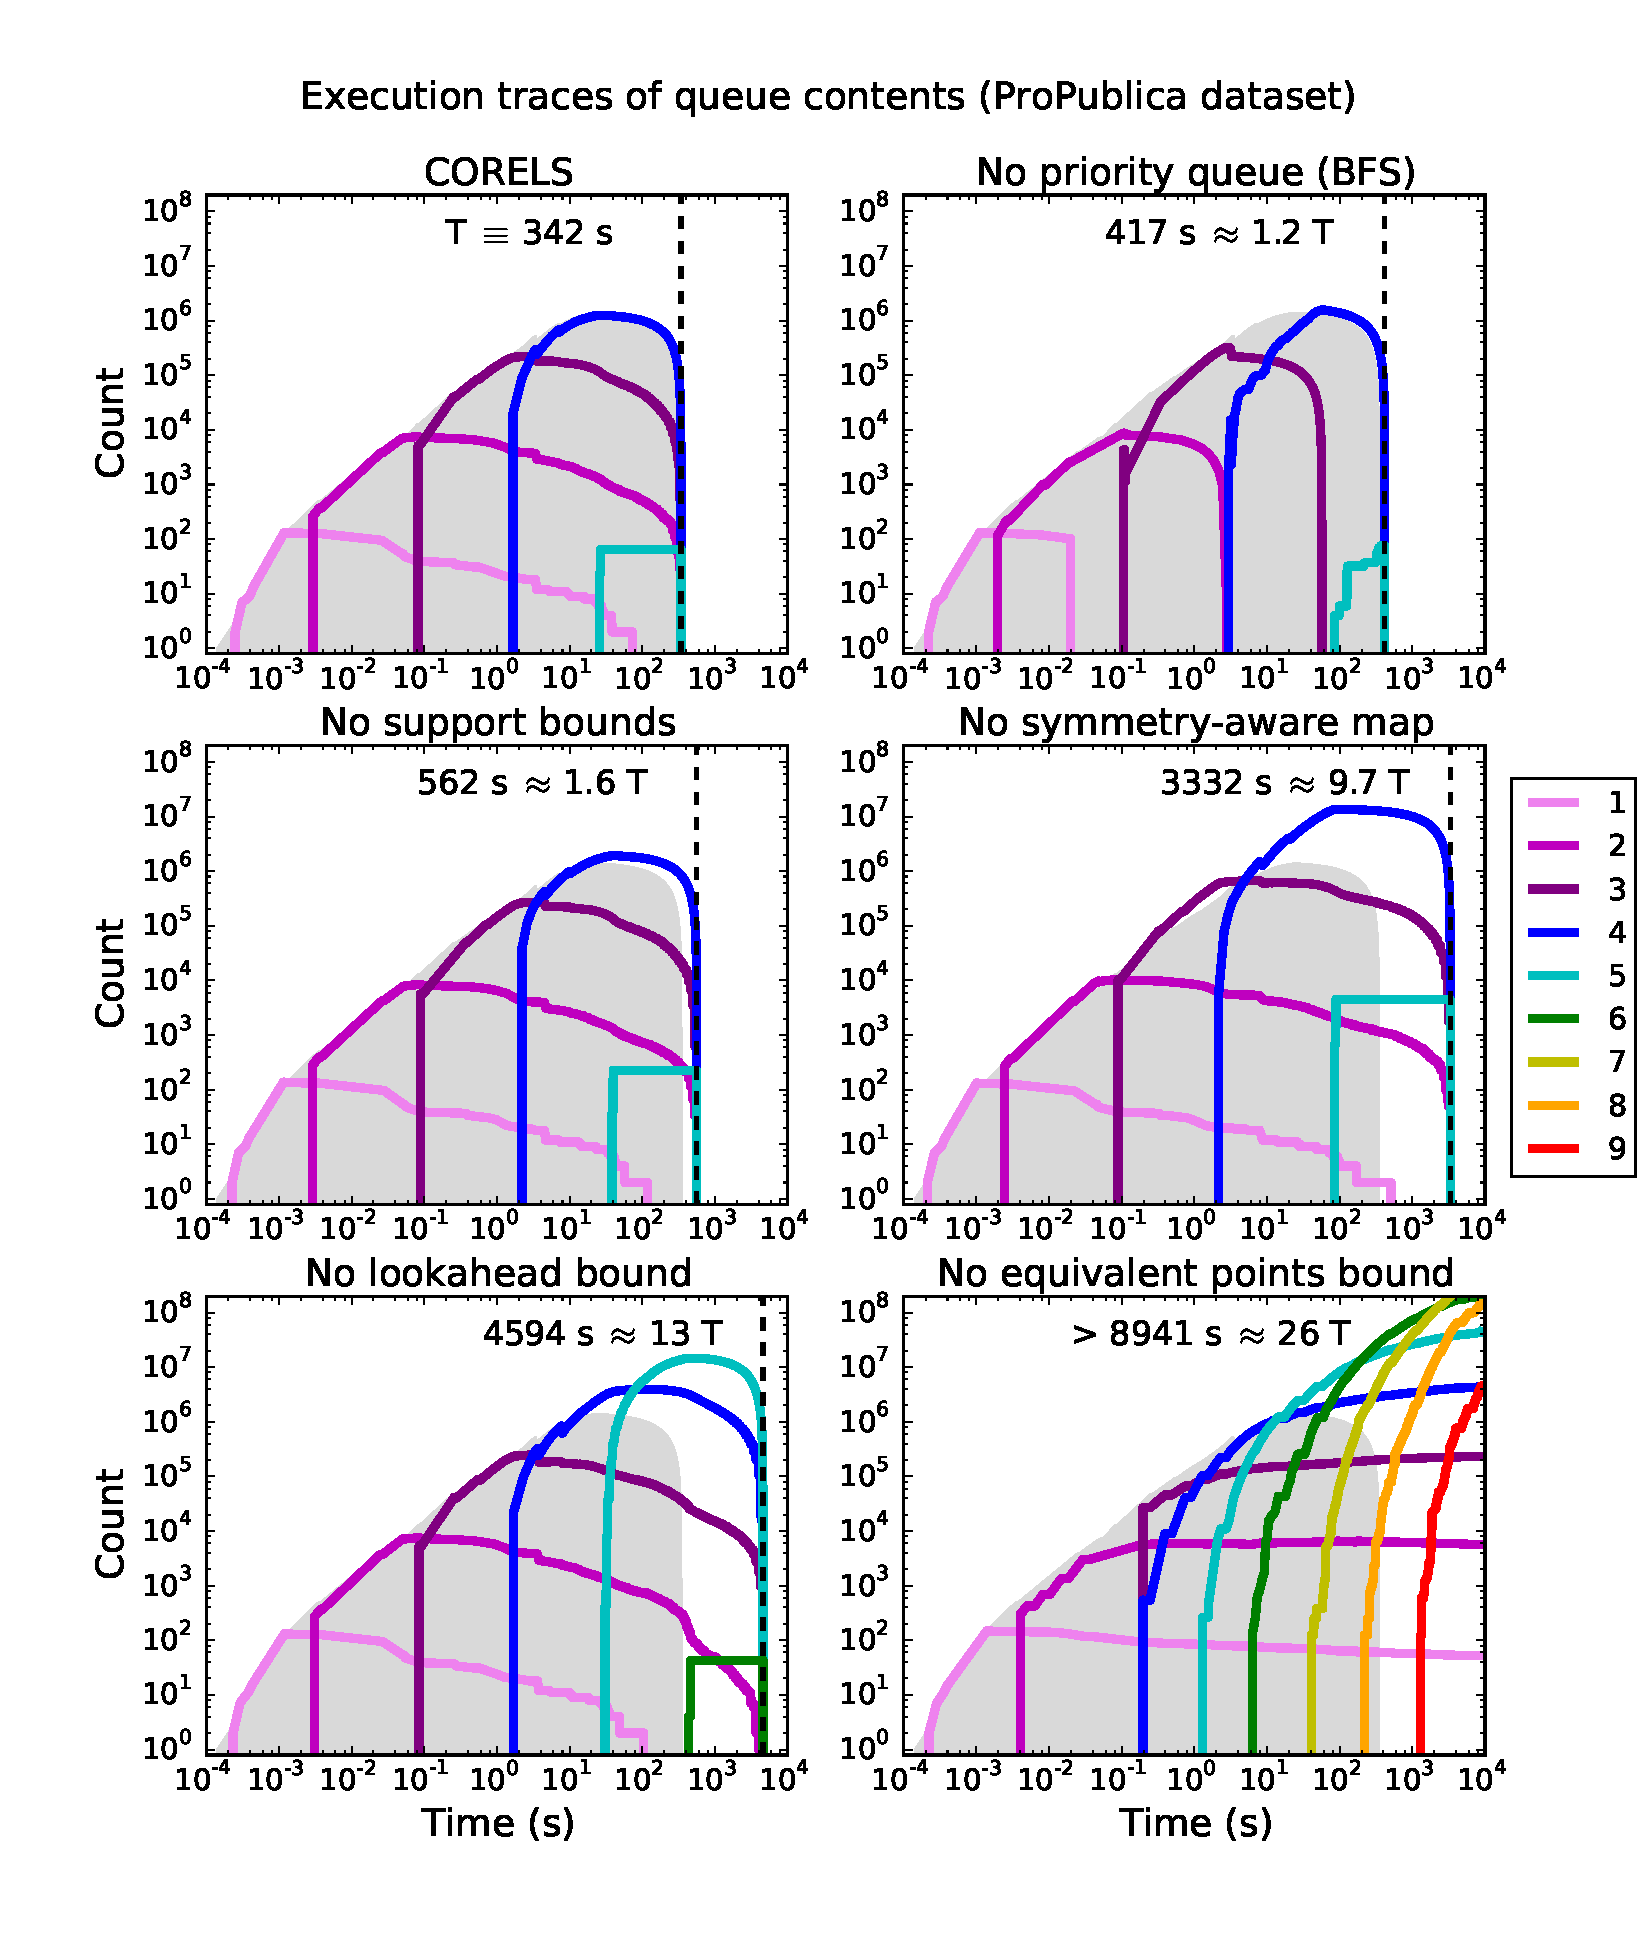
\includegraphics[trim={0mm 10mm 0mm 20mm},
width=0.94\textwidth]{figs/kdd_compas_ablation-queue.pdf}
\end{center}
\vspace{-5mm}
\caption{Summary of the logical queue's contents, for full CORELS (top left)
%\ie the nodes in the physical queue that have not been marked for deletion,
and five variants that each remove a specific implementation optimization or bound,
for the ProPublica dataset (${\Reg = 0.005}$, ${M = 122}$).  See also Table~\ref{tab:ablation}.
%
Solid lines plot the numbers of prefixes in the logical queue (log scale), colored by length (legend),
as a function of wall clock time (log scale).
%
All plots are generated using a single, representative cross-validation training set.
%
The gray shading fills in the area beneath the total number of
queue elements for CORELS,
\ie the sum over all lengths in the top left figure.
%
For comparison, we replicate the same gray region
in the other five subfigures.
%
For each execution, we indicate the total time in seconds,
relative to the full CORELS implementation (T = 304 s),
and with a dashed vertical line.
%
The execution without the equivalent points bound (bottom right) is incomplete.
}
\label{fig:queue}
\end{figure}


Table~\ref{tab:ablation} provides summary statistics for experiments using the full
CORELS implementation and five variants that each remove a specific optimization.
%
(1)~Instead of a priority queue (\S\ref{sec:queue}) ordered by the objective lower bound,
we use a queue that implements breadth-first search (BFS).
%
(2)~We remove checks that would trigger pruning via
our lower bounds on antecedent support (Theorem~\ref{thm:min-capture})
and accurate antecedent support (Theorem~\ref{thm:min-capture-correct}).
%
(3)~We remove the effect of our lookahead bound (Lemma~\ref{lemma:lookahead}),
which otherwise tightens the objective lower bound by~$\Reg$.
%
(4)~We disable the symmetry-aware map (\S\ref{sec:pmap}), our data structure
that enables pruning triggered by the permutation bound (Corollary~\ref{thm:permutation}).
%
(5)~We do not identify sets of equivalent points, which we otherwise use to tighten the
objective lower bound via the equivalent points bound (Theorem~\ref{thm:identical}).

Removing any single optimization increases total execution time,
by varying amounts across these optimizations.
%
Similar to our experiments in~\S\ref{sec:reg-param}, we always encounter the
optimal rule list in far less time than it takes to certify optimality.
%
As in Table~\ref{tab:weapon-reg}, we report metrics that are all proxies
for how much work our algorithm has to do, and thus scale with the overall slowdown.

Figure~\ref{fig:queue} visualizes execution traces of the elements in CORELS's logical queue,
similar to Figure~\ref{fig:queue-weapon-reg},
for a single, representative cross-validation fold.
%
Panels correspond to different removed optimizations, as in Table~\ref{tab:ablation}.
%
These plots demonstrate that our optimizations reduce the number of evaluated prefixes
and are especially effective at limiting the number of longer evaluated prefixes.
%
For the ProPublica dataset, the most important optimization is the equivalent points
bound---without it, we place prefixes of at least length~9 in our queue,
and must terminate these executions before they are complete.
%
In contrast, CORELS, and variants that remove any single one of the other
optimizations evaluate only prefixes up to at most length~7 (without the lookahead bound)
or~6 (all other variants).

Table~\ref{tab:ablation-weapon} and Figure~\ref{fig:queue-weapon} summarize an
analogous set of experiments for the NYCLU dataset.
%
Note that while the equivalent points bound proved to be the most important optimization for the ProPublica dataset,
the symmetry-aware map is the crucial optimization for the NYCLU dataset.

%TODO: UPDATE WITH NEW NUMBERS
\begin{table}[t!]
\centering
%\begin{centering}
Per-component performance improvement (NYCLU stop-and-frisk dataset) \\
%\end{centering}
\vspace{1mm}
\begin{tabular}{l | c  r | c | c}
& Total & Slow- & Time to & Max evaluated \\
Algorithm variant & time (min) & down & optimum ($\mu$s) & prefix length \\
\hline
CORELS & .7 (.1) & --- & 6.7 (.1) & 11 \\
No priority queue (BFS) & 1.5 (.1) & 2.0$\times$ & 60 (20) & 11 \\
No support bounds & 1.4 (.1) & 1.9$\times$ & 10 (.1) & 11-12 \\
No lookahead bound & 1.2 (.1) & 1.6$\times$ & 6.9 (.3) & 11-12 \\
No symmetry-aware map & 620 (100) & 850$\times$ & 6.6 (.1) & 11 \\
No equivalent points bound & 2.4 (.1) & 3.4$\times$ & 6.0 (.4) & 13 \\
\hline
\end{tabular}
\begin{tabular}{l | c | c | c}
\hline
 & Lower bound & Total queue &  Max queue \\
Algorithm variant & evaluations ($\times 10^6$) & insertions ($\times 10^5$) & size ($\times 10^5$) \\
\hline
CORELS & 6.0 (.5) & 1.7 (.1) & 1.0 (.1) \\
No priority queue (BFS) & 12 (1) & 3.6 (.3) & 1.3 (.1) \\
No support bounds & 11 (1) & 3.1 (.3) & 1.8 (.1) \\
No lookahead bound & 9.6 (.7) & 2.8 (.2) & 1.7 (.1) \\
No symmetry-aware map & 5200 (800) & 1400 (200) & 1100 (200) \\
No equivalent points bound & 26 (1) & 7.5 (.4) & 4.5 (.2) \\
\end{tabular}
%\vspace{4mm}
\caption{Per-component performance improvement, as in Table~\ref{tab:ablation},
for the NYCLU stop-and-frisk dataset (${\Reg = 0.01}$, ${M = 46}$).
%
All rows represent complete executions.
%
See Table~\ref{tab:ablation} for a detailed caption,
and also Figure~\ref{fig:queue-weapon}.
}
\vspace{4mm}
\label{tab:ablation-weapon}
\end{table}

%TODO: UPDATE WITH ABLATION
\begin{figure}[t!]
\begin{center}
% left lower right upper
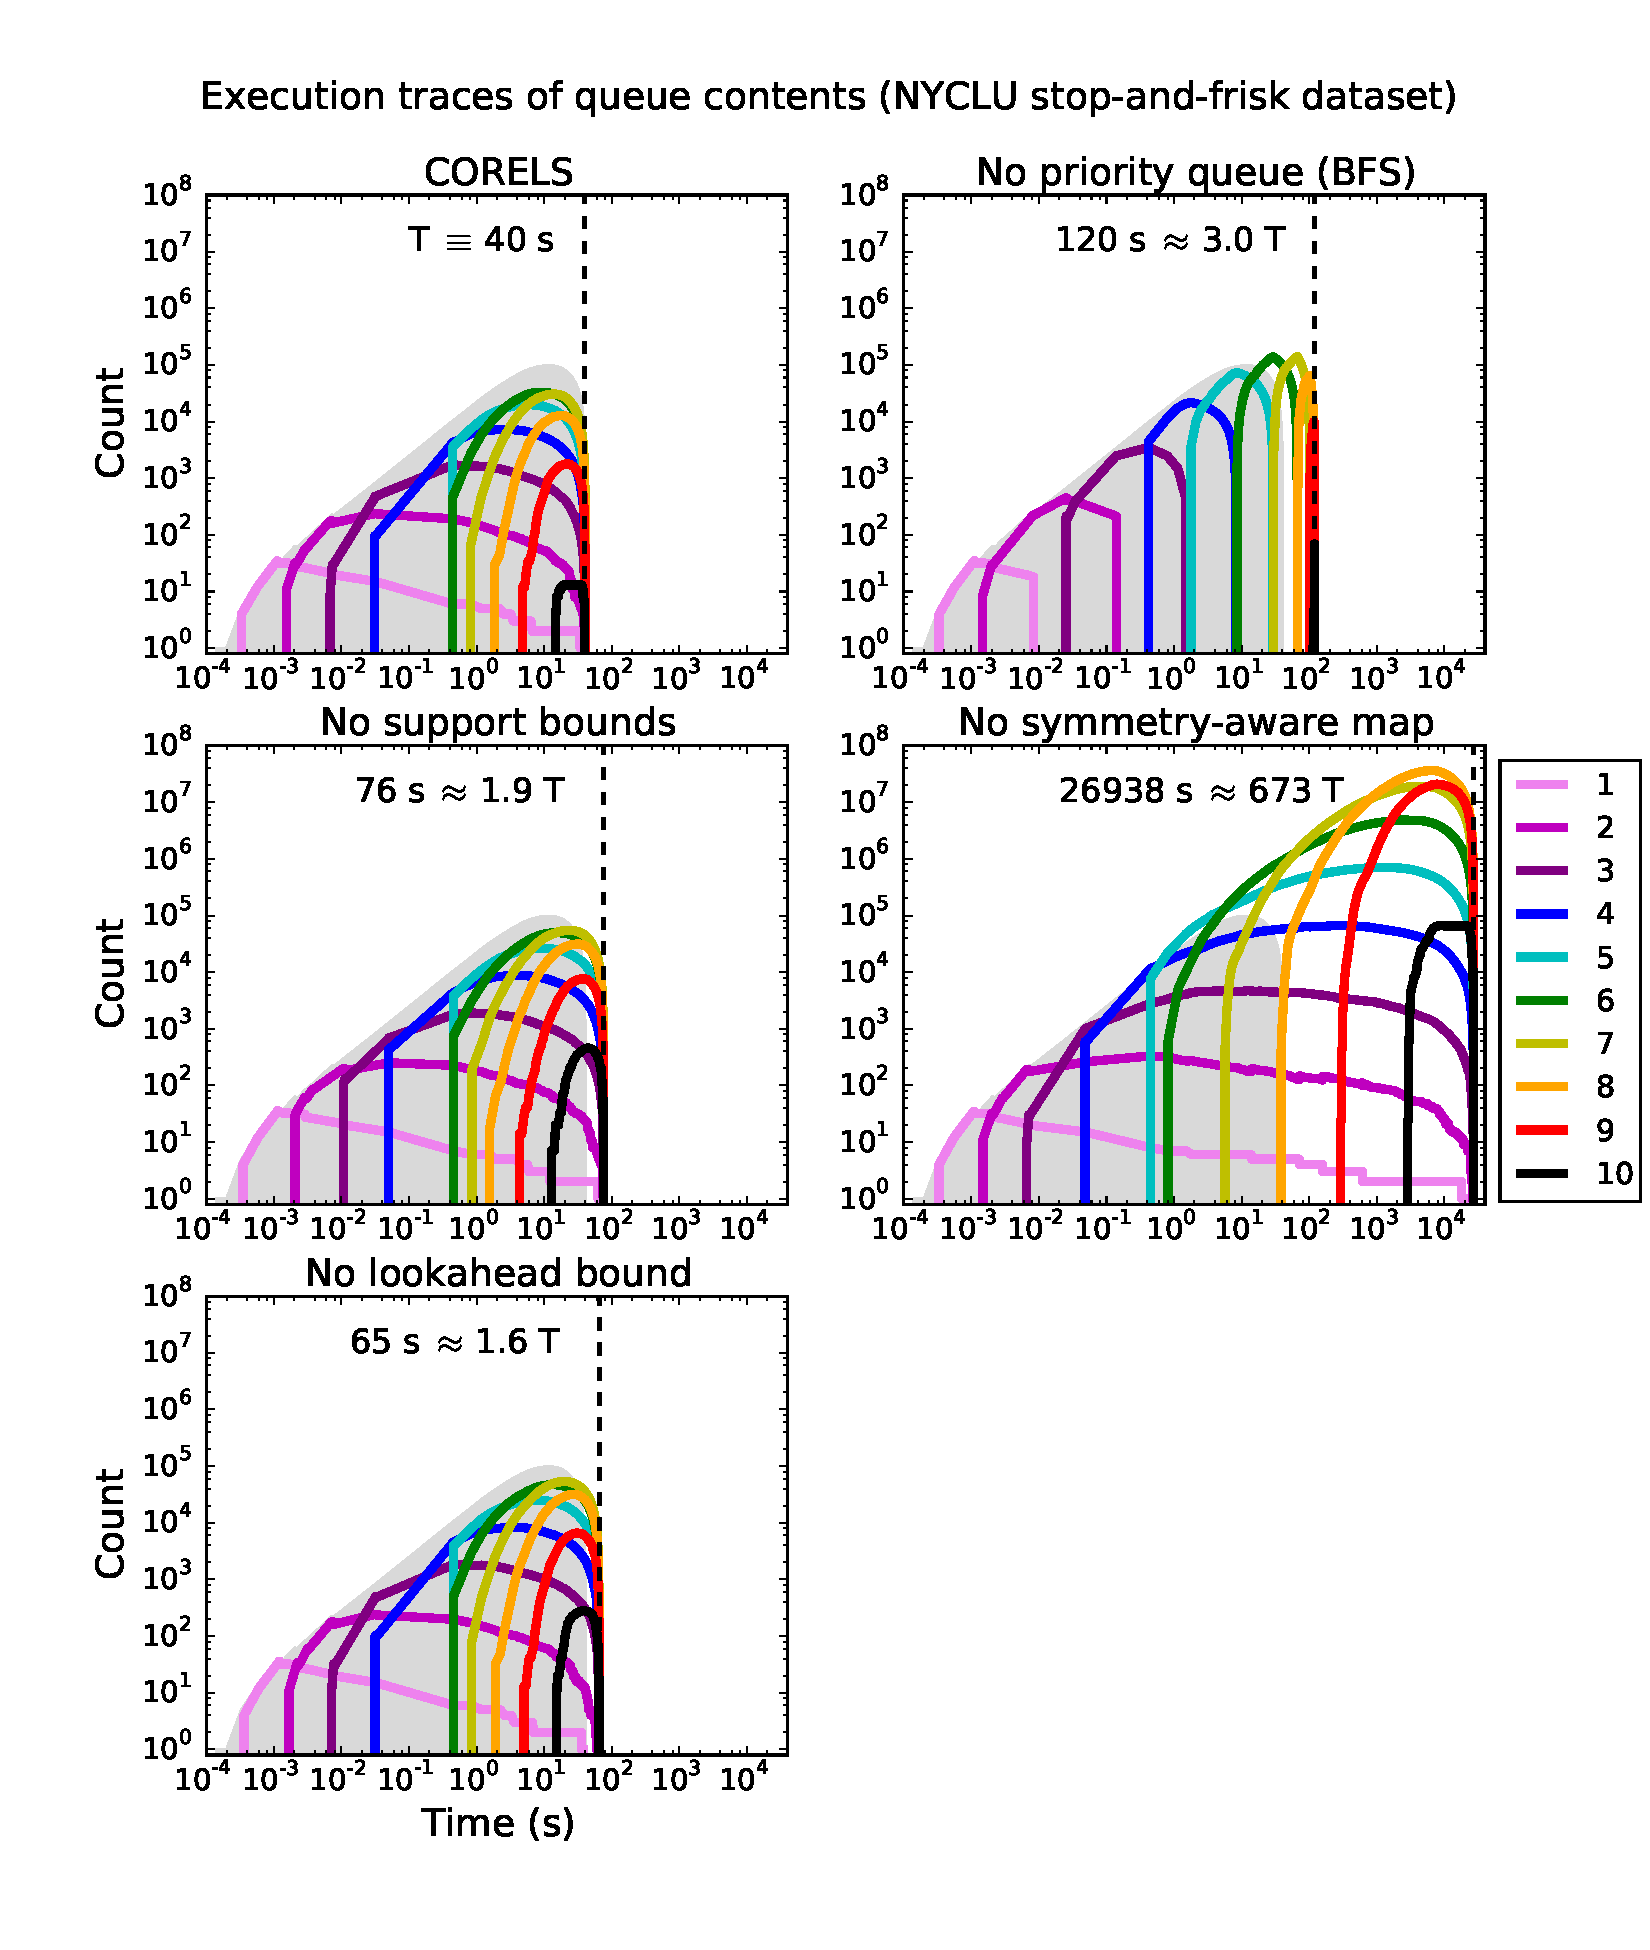
\includegraphics[trim={0mm 10mm 0mm 20mm},
width=0.94\textwidth]{figs/weapon_ablation-queue.pdf}
\end{center}
\vspace{-5mm}
\caption{Summary of the logical queue's contents, for full CORELS (top left)
and five variants that each remove a specific implementation optimization or bound,
for the NYCLU stop-and-frisk dataset (${\Reg = 0.01}$, ${M = 46}$), as in Table~\ref{tab:ablation-weapon}.
%
See Figure~\ref{fig:queue} for a detailed caption.
}
\label{fig:queue-weapon}
\end{figure}

Finally, Figure~\ref{fig:objective} highlights the most significant
algorithm optimizations for our prediction problems:
the equivalent points bound for the ProPublica dataset (left)
and the symmetry-aware map for the NYCLU dataset (right).
%
For CORELS (thin lines) with the ProPublica recidivism dataset (left),
the objective drops quickly, achieving the optimal value within 10 seconds.
CORELS certifies optimality in less than 6 minutes --
the objective lower bound steadily converges to the optimal objective (top)
as the search space shrinks (bottom).
%
As in Figure~\ref{fig:weapon-reg-execution}, we dynamically and incrementally
calculate~$\lfloor \log_{10} \Remaining(\CurrentObj, \Queue) \rfloor$,
where~$\Remaining(\CurrentObj, \Queue)$
is the upper bound~\eqref{eq:remaining} on remaining search space size
(Theorem~\ref{thm:remaining-eval-fine}); this adds some computational overhead.
%
In the same plots (left), we additionally highlight
a separate execution of CORELS without the equivalent points bound
(Theorem~\ref{thm:identical}) (thick lines).
%
After nearly 3 hours, the execution is still far from complete;
in particular, the lower bound is far from the optimum objective value (top)
and much of the search space remains unexplored (bottom).
%
For the NYCLU stop-and-frisk dataset (right),
CORELS achieves the optimum objective in well under a second,
and certifies optimality in less than a minute.
%
CORELS without the permutation bound (Corollary~\ref{thm:permutation}),
and thus the symmetry-aware map,
requires orders of magnitude more time to complete (thick lines).

%TODO UPDATE WITH NO IMPORTANT BOUND
\begin{figure}[t!]
\begin{center}
%\includegraphics[width=0.65\textwidth]{figs/sketch-objective.png}
% left lower right upper
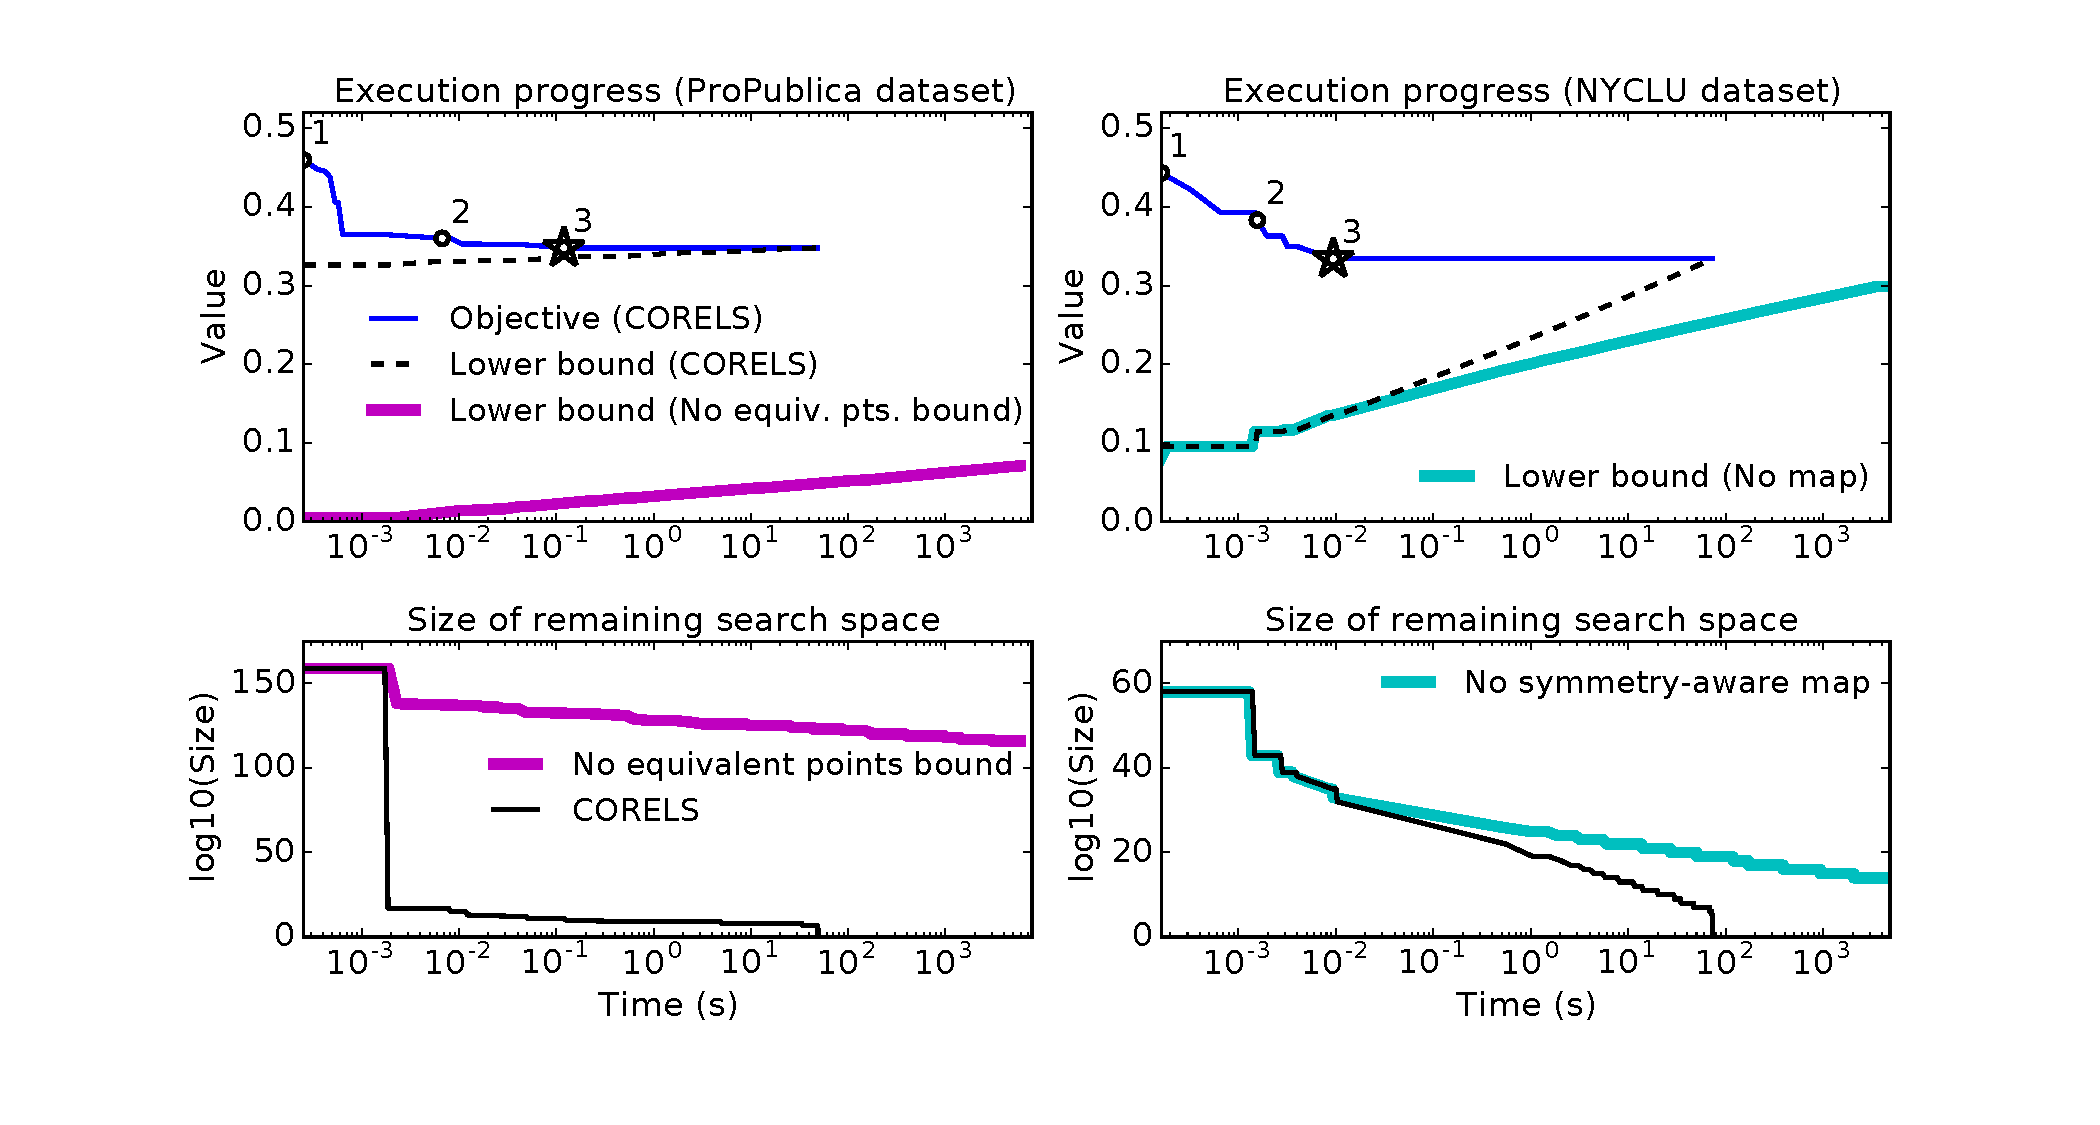
\includegraphics[trim={30mm, 20mm, 30mm, 20mm},
width=\textwidth]{figs/weapon_execution_large-remaining-space.pdf}
\end{center}
\caption{Execution progress of CORELS and selected variants,
for the ProPublica (${\Reg = 0.005}$, ${M = 122}$) (left)
and NYCLU (${\Reg = 0.01}$, ${M = 46}$) (right) datasets.
%
Top: Objective value (thin solid lines) and lower bound (dashed lines) for CORELS,
as a function of wall clock time (log scale).
%
Numbered points along the trace of the objective value
indicate when the length of the best known rule list changes,
and are labeled by the new length.
%
CORELS quickly achieves the optimal value (star markers),
and certifies optimality when the lower bound matches the objective value.
%
On the left, a separate and significantly longer execution of CORELS
without the equivalent points  (Theorem~\ref{thm:identical}) bound remains
far from complete, and its lower bound (thick solid line) far from the optimum.
%
On the right, a separate execution of CORELS without the permutation bound
(Corollary~\ref{thm:permutation}), and thus the symmetry-aware map,
requires orders of magnitude more time to complete.
%
Bottom: $\lfloor \log_{10} \Remaining(\CurrentObj, \Queue) \rfloor$,
as a function of wall clock time (log scale),
where~$\Remaining(\CurrentObj, \Queue)$
is the upper bound~\eqref{eq:remaining} on remaining search space size
(Theorem~\ref{thm:remaining-eval-fine}).
%
For these problems, the equivalent points (left) and
permutation (right) bounds are responsible for the ability of
CORELS to quickly eliminate most of the search space (thin solid lines);
the remaining search space decays much more slowly without these bounds (thick solid lines).
}
\label{fig:objective}
\end{figure}

\subsection{Algorithmic Speedup}
%
We calculate the overall speed-up of CORELS compared to a naive implementation and determine the feasibility of running
our algorithm 30 years ago.
%
Consider an execution of CORELS for the ProPublica dataset, with ${M = 122}$ antecedents,
that evaluates prefixes up to length~5 in order to certify optimality (Table~\ref{tab:ablation}).
%
A brute force implementation that naively considers all prefixes of up to length~5
would evaluate ${2.5 \times 10^{10}}$ prefixes.
%
As shown in Figure~\ref{fig:recidivism-all-folds}, the optimal rule list has prefix length~4,
thus the brute force algorithm would identify the optimal rule list.
%
However, for this approach certify optimality, it would have consider far longer prefixes.
%
Without our equivalent points bound, but with all of our other optimizations,
we evaluate prefixes up to at least length 10
(see Table~\ref{tab:ablation} and Figure~\ref{fig:queue})---thus a brute force algorithm
would have to evaluate prefixes of length 10 or longer.
%
Naively evaluating all prefixes up to length 10 would require looking at $5.0 \times 10^{20}$ different prefixes.
%
However, CORELS examines only 28 million prefixes in total---a reduction of $1.8 \times 10^{13}$.
%
It takes us about 2$\mu$s to evaluate a single prefix (given by dividing the number of lower bound evaluations by the total time
in Table~\ref{tab:ablation}).
%
A naive solution would take $1.54 \times 10^8$ seconds---about 5 years---while CORELS takes less than a minute.
%
It is clear that brute force would not scale to larger problems.
%

We compare our current computing circumstances to those of 1984, the year when CART was published.
%
Moore's law holds that computing power doubled every 18 months from 1984-2006.
%
This is a period of 264 months, which means computing power has gone up by at least a factor of $32,000$ since 1984.
%
Thus, even with our algorithmic and data structural improvements, CORELS would have run in over 1,792,000s in 1984---an unreasonable amount of time.
%
Our advances are meaningful only because we can run them on a modern system.
%
Combining our algorithmic improvements with the increase in modern processor speeds, our algorithm runs more than $10^{18}$ times faster than a naive implementation would have in 1984.
%
This helps explain why our algorithm, nor other branch-and-bound variants, had not been developed before now.
